\ifdefined \wholebook \else\documentclass[oneside]{book}\usepackage{EdlBook}\graphicspath{{figures/}}
\addto\captionsicelandic{\renewcommand{\chaptername}{Kafli}}
%\setsecnumdepth{chapter}
\begin{document}
%%%
%
\setcounter{chapter}{13} % one less than this chapter
%
%%%
\fi
%%%%%%%%%%%%%%%%%%%%%%%%%%%%%%%%
%      CHAPTER TEXT GOES BELOW
%%%%%%%%%%%%%%%%%%%%%%%%%%%%%%%%

\renewcommand{\thefigure}{\arabic{figure}}
\counterwithout{equation}{chapter}


\chapter{Rafsviðið}


Forngríska heimspekingnum Demókrítus (400 f.Kr) hefur oft verið eignuð atómkenningin, það er að segja kenningin sem segir að allt efni samanstandi af litlum frumeindum eða atómum sem eru minnsta eining sem hægt er að skipta efni niður í. Bandaríski eðlisfræðingurinn (og Nóbelsverðlaunahafinn) Richard P. Feynman segir í upphafi fyrirlestra sinna\footnote{\href{https://www.feynmanlectures.caltech.edu/}{Hlekkur á Feynman fyrirlestrana á netinu}}:

\blockquote{\educk{If, in some cataclysm, all of scientific knowledge were to be destroyed, and only one sentence passed on to the next generations of creatures, what statement would contain the most information in the fewest words? I believe it is the atomic hypothesis (or the atomic fact, or whatever you wish to call it) that all things are made of atoms—little particles that move around in perpetual motion, attracting each other when they are a little distance apart, but repelling upon being squeezed into one another. In that one sentence, you will see, there is an enormous amount of information about the world, if just a little imagination and thinking are applied.} \\ \phantom{.} \hfill \textbf{- \, Richard P. Feynman}}

Í ár ætlum við að reyna að rannsaka þetta atómlíkan og reyna að varpa ljósi á þær breytingar sem hafa orðið í gegnum tíðina á hugmyndum eðlisfræðinga um atómið. Fyrir jól munum við einblína á rafsegulkraftinn. Honum er lýst af Maxwellsjöfnunum fjórum (já, við þurfum bara að læra fjórar jöfnur fyrir jól!) sem settar voru fram af skoska eðlisfræðingnum James Clerk Maxwell árið 1865. Skilningur mannkynsins á Maxwellsjöfnunum fjórum hefur fært okkur öll þau helstu nútímaþægindi sem að við höfum tekið að venjast - þær eru lykillinn að því að skilja öll þau raftæki sem að við notum í okkar daglega lífi (eins og t.d.~snjallsímana okkar). \\

Eftir jól munum við skoða takmörkuðu afstæðiskenningu Einsteins og kafa dýpra í atómlíkanið þar sem að við munum sjá fyrstu merki þess að Newtonska eðlisfræðin sem við höfum lært hingað til er ekki fær um að lýsa því sem á sér stað inni í atóminu. Til þess þurfum við skammtafræði. Skammtafræðin setur ákveðnar skorður á heiminn sem að við búum í. Hún segir að ákveðnir hlutir (t.d.~orka) komi í \emph{skömmutum} og geti því ekki tekið hvaða gildi sem er heldur einungis heiltölumargfeldi af minnsta gildi stærðarinnar. Þetta hefur gríðarlegar afleiðingar þrátt fyrir það að þetta kunni að hljóma eins og að það skipti voða litlu máli! En það að hlutir séu skammtaðir ætti ekki að vera nýtt af nálinni - því það er einmitt það sem að atómkenningin segir: Að allt efni samanstandi af litlum óþættanlegum frumeindum sem er minnsta eining alls efnis. \\



Vegferð okkar í vetur byrjar á því að skoða einfalt líkan af atóminu þar sem að í miðju atómsins er kjarni þar sem að allar róteindirnar og niteindirnar hafa pakkað sér þétt saman. Langt í burtu frá þeim eru rafeindir á hringhreyfingu umhverfis kjarnann. Fyrir vetnisatómið sem að samanstendur af einni róteind og einni rafeind lítur þetta svona út:


\begin{figure}[H]
    \centering
    \begin{tikzpicture}
        \draw [line width = 0.8pt] (5, 2) arc [radius=2cm, start angle=0, delta angle=360];
        \draw[dashed] (3,2) -- (4.4,0.45);
        \filldraw[draw=black] (1,1.9) circle (0.15cm);
        \filldraw[draw=black] (3,2) circle (0.2cm);
        \node at (0.5,2.1) {\(m_e\)};
        \node at (0.65,1.25) {\(v\)};
        \node at (1.3,2.2) {\(-e\)};
        \node at (3.4,2.3) {\(m_p\)};
        \node at (2.55,2.4) {\(+e\)};
        \node at (3.4,1) {\(a_0\)};
        \draw[thick, -Stealth] (0.975,1.9) -- (0.975,1);
        \node at (10,4) {Massi rafeindar: $m_e = \SI{9.11e-31}{kg}$};
        \node at (10,3.5) {Massi róteindar: $m_p = \SI{1.67e-27}{kg}$};
        \node at (10,3) {Massi nifteindar: $m_n = \SI{1.67e-27}{kg}$};
        \node at (10,2.5) {Frumeindamassinn: $u = \SI{1.66e-27}{kg}$};
        \node at (10,1.5) {Geisli róteindar: $r_p = \SI{0.85e-15}{m}$};
        \node at (10,1) {Geisli atómsins: $a_0 = \SI{5.29e-11}{m}$};
        \node at (10,0) {Grunnhleðslan: $e = \SI{1.602e-19}{C}$};
    \end{tikzpicture}
    \caption{Einfalt líkan af vetnisatóminu.}
\end{figure}

Þetta minnir svolítið á líkani okkar fyrir plánetu á hringhreyfingu umhverfis sólina. Þetta líkan af atóminu er ágætt sem tól til þess að ímynda sér uppbyggingu atómsins. En það hefur þó nokkra galla sem að við munum reyna að varpa ljósi á þegar líður á árið. Nokkrir hlutir sem að þið ættuð að taka eftir. Í fyrsta lagi er $u \approx m_p \approx m_n$ en síðan sjáum við líka að:
\begin{align*}
    \frac{m_p}{m_e} \approx 2000, \hspace{1cm} \text{svo róteindir og nifteindir eru mun massameiri heldur en rafeindir.}
\end{align*}
Stærðin á kjarnanum er af stærðargráðunni $\SI{e-15}{m}$ þ.e.~\si{fm}, en stærðin á atóminu er af stærðargráðunni $\SI{e-10}{m}$ þ.e.~\si{\angstrom} (til heiðurs sænska eðlisfræðingnum Anders Jonas Ångström). Þetta þýðir að rúmmál kjarnans er afar lítið í samnburði við stærð atómsins.\\

Annað sem að við ættum að nefna er í tengslum við grunnhleðsluna. Rafeindir hafa neikvæða hleðslu $-e = \SI{-1.602e-19}{C}$ og róteindir hafa jákvæða hleðslu $+e = \SI{+1.602e-19}{C}$. Hinsvegar hafa nifteindir enga hleðslu. Hleðslan, $e$, kallast \emph{grunnhleðslan} því að það er minnsta einingin á hleðslu sem að við getum haft. Þetta hefur afar djúpstæðar afleiðingar, því þetta þýðir að hleðsla er skömmtuð stærð (sbr. skammtafræði):

\begin{tcolorbox}
\begin{definition}
Við segjum að hleðsla sé \emph{\textbf{skömmtuð}} því ef við erum með einhvern hlut sem hefur hleðslu $q$ þá þarf $q$ að vera heiltölu margfeldi af grunnhleðslunni, það er að segja til er $n \in \Z$ þannig að:
\begin{align*}
    q = n \cdot e, \hspace{2cm} e = \SI{1.602e-19}{C}.
\end{align*}
\end{definition}

\end{tcolorbox}

En við höfðum séð að ef hlutur er á hringhreyfingu þá verkar á hann miðsóknarkraftur, þ.e.~heildarkrafturinn sem að verkar á hlutinn er inn að miðju hringsins.

\begin{figure}[H]
    \centering
    \begin{tikzpicture}
        \draw [line width = 0.8pt] (5, 2) arc [radius=2cm, start angle=0, delta angle=360];
        \draw[dashed] (3,2) -- (4.4,0.45);
        \filldraw[draw=black] (5,1.9) circle (0.15cm);
        \filldraw[draw=black] (3,2) circle (0.2cm);
        \node at (5.5,1.7) {\(m_e\)};
        \node at (5.35,2.6) {\(v\)};
        \node at (4.5,1.5) {\(-e\)};
        \node at (2.55,1.5) {\(m_p\)};
        \node at (2.55,2.4) {\(+e\)};
        \node at (4.3,2.3) {\(F_{\text{heild}}\)};
        \node at (3.4,1) {\(r\)};
        \draw[thick, -Stealth] (5,1.9) -- (3.75,1.9);
        \draw[-Stealth] (5.05,1.9) -- (5.05,2.75);
    \end{tikzpicture}
    \caption{Heildarkrafturinn liggur inn að miðju hringsins í einsleitri hringhreyfingu.}
\end{figure}

En hvaða kraftur er þetta sem að heldur rafeindinni á hringhreyfingu um róteindina? Við gætum til að byrja með haldið að þetta væri þyngdarlögmálskrafturinn:
\begin{align*}
    F_G = \frac{Gm_1m_2}{r^2}, \hspace{2cm} G = \SI{6.67e-11}{Nm^2/kg^2}
\end{align*}
En við sjáum fljótt að þá hefðum við að (við rifjum upp að miðsóknarhröðunin er $a_{\text{mið}} = \frac{v^2}{r}$):
\begin{align*}
    m \frac{v^2}{r} = \frac{Gm_e m_p}{r^2} \implies v = \sqrt{\frac{Gm_p}{r}} = \sqrt{\frac{\SI{6.67e-11}{}\cdot \SI{1.67e-27}{}}{\SI{5.29e-11}{}}} \approx \SI{e-14}{m/s}.
\end{align*}
Sem er alltof lítill hraði fyrir rafeindina! Rafeindir sniglast ekki svona áfram! Þannig það hlítur að vera annar kraftur sem að heldur rafeindunum á hringhreyfingu! Hvaða kraftur er það? Það er Coulombskrafturinn!


\section{Rafkraftalögmál Coulombs}

\begin{tcolorbox}
\begin{theorem}
\textbf{(Lögmál Coulombs)} Lítum á tvær hleðslur $q_1$ og $q_2$. Látum $\Vec{r}$ vera vigur á milli þeirra sem hefur lengd $r$, sem er fjarlægðin milli hleðslanna. Látum $\Vec{e}_{\vec{r}}$ tákna einingarvigur vigursins $\Vec{r}$. Þá verkar á milli þeirra rafkraftur sem er gefinn með:
\begin{align*}
    \vec{F}_k = \frac{kq_1 q_2}{r^2} \Vec{e}_{\vec{r}}
\end{align*}
Þar sem $k = \SI{9.0e9}{Nm^2/C^2}$ er fasti sem nefnist fasti Coulombs. Krafturinn er aðdráttarkraftur ef $q_1$ og $q_2$ hafa gagnstæð formerki en fráhrindikraftur ef $q_1$ og $q_2$ hafa sama formerki.
\end{theorem}
\end{tcolorbox}

Stundum er reyndar Coulombs-fastinn táknaður við annan fasta sem nefnist \textit{rafsvörunarstuðull tómarúms}, $\varepsilon_0$ (nánar um hann síðar og af hverju fólk vill gera það). Þá skrifar fólk stundum að:
\begin{align*}
    k = \frac{1}{4\pi \varepsilon_0}, \hspace{1cm} \text{þar sem} \hspace{0.5cm} \varepsilon_0 = \SI{8.85e-12}{s^2.C^2/(kg.m^3)}
\end{align*}


Ef við skoðum Coulombskraftinn nánar þá sjáum við að $F_k \gg F_G$ inni í atóminu\footnote{Táknið $\gg$ þýðir að stærðin sem er vinstra megin er miklu stærri heldur en stærðin sem er hægra meginn.}. Því þar gildir:
\begin{align*}
    \frac{F_k}{F_G} = \frac{\frac{ke^2}{r^2}}{\frac{Gm_em_p}{r^2}} = \frac{k}{G} \cdot \frac{e^2}{m_e m_p} = \frac{\SI{9e9}{}}{\SI{6.67e-11}{}} \cdot \frac{(\SI{1.602e-19}{})^2}{(\SI{1.67e-27}{})(\SI{9.11e-31}{})} \approx 10^{9-2\cdot19 + 11 + 27+31} = 10^{40}.
\end{align*}
Þannig að í þessu samhengi þá skiptir þyngdarlögmálskrafturinn engu máli í samanburði við Coulombskraftinn. Almennt gildir að við getum oftast hunsað þyngdarlögmálskraftinn í öllum þeim reikningum sem að við gerum þegar að rafkrafturinn er til staðar. Rafkrafturinn er einfaldlega miklu miklu sterkari heldur en þyngdarlögmálskrafturinn. En þá höfum við fyrir hringhreyfingu rafeindarinnar um róteindina að:
\begin{align*}
    m_e \frac{v^2}{r} = \frac{ke^2}{r^2} \implies v = \sqrt{\frac{ke^2}{m_e r}} = e \cdot \sqrt{\frac{k}{m_e r}} = \SI{1.602e-19}{} \cdot \sqrt{\frac{\SI{9e9}{}}{\SI{9.11e-31}{}\cdot \SI{5.29e-11}{}}} \approx \SI{e-6}{m/s}.
\end{align*}
Sem er frekar eðlilegur hraði miðað við að rafeindir ferðast hratt en þó hægar heldur en ljósið. \\

Coulombskrafturinn og þyngdarlögmálskrafturinn eru afar líkir - helsti munurinn felst í því að hleðslur geta haft mismunandi formerki (þær geta verið jákvæðar eða neikvæðar) en massar (eins og við þekkjum þá) geta einungis verið jákvæðir. Þetta gerir það að verkum að Coulombskrafturinn getur haft tvær stefnur. Hann er aðdráttarkraftur ef hleðslurnar hafa gagnstætt formerki ($+$ og $-$) en hann er fráhrindikraftur ef að hleðslurnar hafa sama formerki ($+$ og $+$) eða ($-$ og $-$). \\

\section{Rafsvið frá punkthleðslu}

Spurningin sem að við viljum reyna að svara í rafsegulfræði er eftirfarandi:

\blockquote{\educk{Ef ég er með hleðslur: $Q_1, Q_2, \ldots, Q_n$ sem hafa einhverja staðsetningu, hraða, hröðun og massa. Get ég þá spáð fyrir því hvering einhver önnur hleðsla, $q$, (köllum hana \textbf{prufuhleðsluna}) mun hreyfast vegna hinna?\phantom{.}} \\ \phantom{.} \hfill \textbf{}}


\begin{figure}[H]
    \centering
    \begin{tikzpicture}
        \draw (3,2) circle (0.35cm);
        \node at (3,2) {\(Q_1\)};
        \draw (2.2,1.2) circle (0.35cm);
        \node at (2.2,1.2) {\(Q_2\)};
        \draw (3.3,1.25) circle (0.35cm);
        \node at (3.3,1.25) {\(Q_n\)};
        \draw (7.5,1.5) circle (0.30cm);
        \node at (7.5,1.5) {\(q\)};
        \node at (8.5,2.2) {\emph{Prufuhleðsla}};
    \end{tikzpicture}
    \caption{Hvernig mun hleðslan $q$ hreyfast vegna $Q_1, Q_2, \ldots, Q_n$?}
\end{figure}

En, höfum við ekki nú þegar leyst þetta vandamál? Við höfum einfaldlega að heildarkrafturinn sem að verkar á $q$ er gefinn með:
\begin{align*}
    \vec{F}_{\text{heild}} &= \vec{F}_1 + \vec{F}_2 + \ldots + \vec{F}_n \\
    &= \frac{kqQ_1}{r_1^2} \hat{\vec{r}}_1 + \frac{kqQ_2}{r_2^2} \hat{\vec{r}}_2 + \ldots + \frac{kqQ_n}{r_n^2} \hat{\vec{r}}_n.
\end{align*}

Þar sem að $\vec{r}_n$ er vigurinn frá $Q_n$ til $q$, $r_n = \abs{\vec{r}_n}$ og $\hat{\vec{r}}_n = \frac{\vec{r}_n}{r_n}$ er einingarvigurinn.

En í rafsegulfræði þá erum við að glíma við mikinn fjölda af eindum þannig að fjöldi liða getur orðið mjög stór (af sömu stærðargráðu og Avogadrosartalan $N_A = \SI{6.022e23}{}$!). Hvert okkar samanstendur af billjónum af frumum og hver þeirra samanstendur af billjónum af atómum og hvert þeirra samanstendur af nokkrum rafeindum og róteindum. Það er engin leið fyrir okkur til þess að lýsa öllum þessum eindum með rafkröftum Coulombs. Við þyrftum að gera billjón billjónir af kraftamyndum og það er því algjörlega ómögulegt fyrir okkur að ætlast til þess að við getum bara skrifað niður heildarkraftinn fyrir prufuhleðsluna, $q$ og sagst hafa leyst vandamálið! Við þurfum nýja leið til þess að sjá heiminn! Nýja og öflugari leið til þess að hugsa um eðlisfræðileg fyrirbæri. Lausnin á þessu vandamáli felst í því að skoða svokallað sviðshugtak (e. \emph{field}) sem lýsir því hvernig hlutir hreyfast út frá því hvar þeir eru staddir. Til dæmis þá vitum við að epli fellur niður í áttina að jörðinni vegna þyngdarsviðsins. Svið og kraftur eru því afar náskyld hugtök og við munum reyna á þessari önn að skýra í hverju munurinn felst. Sviðshugtakið er oftast kennt við Breska vísindamanninn Michael Faraday, en það er sérlega athyglisvert því hann hafi litla kunnáttu í stærðfræði og var ekki skólagenginn maður. Það er vegna þess að sviðshugtakið hefur bæði stærðfræðilega skilgreiningu og myndræna skilgreiningu (Faraday notaði þá síðari).

\begin{tcolorbox}
\begin{definition}
\textbf{(Rafsvið frá punkthleðslu)} Lítum á punkthleðslu $Q$. Ímyndum okkur að við komum lítilli prufuhleðslu $q$ fyrir í fjarlægð $r$ frá punkthleðslunni. Látum vigurinn á milli þeirra vera $\Vec{r}$. Þá er \textbf{rafsviðið}, $\vec{E}$, sem að prufuhleðslan $q$ finnur fyrir vegna punkthleðslunnar $Q$ gefið með:
\begin{align*}
    \Vec{E} = \frac{\vec{F}_k}{q}= \frac{kQ}{r^2} \hat{\vec{r}}.
\end{align*}
\end{definition}
\end{tcolorbox}

Stærðfræðilega lítur út eins og að við séum ekki að gera mikið en hugmyndafræðilega þá er þetta afar öflug leið til þess að hugsa um heiminn! En ég lofaði líka að gefa myndræna skilgreiningu:


\begin{tcolorbox}
Við teiknum rafsviðslínur frá punkthleðslu þannig að þær gefi til kynna í hvaða stefnu jákvæð prufuhleðsla, $+q$, myndi ferðast ef henni væri sleppt af stað nálægt punkthleðslunni. Það þýðir að rafsviðslínurnar frá jákvæðum punkthleðslum eru í burtu frá henni en rafsviðslínur frá neikvæðum punkthleðslum eru að henni. Styrkur rafsviðsins er táknaður með því hversu þéttar rafsviðslínurnar eru á myndinni.
\begin{figure}[H]
    \centering
    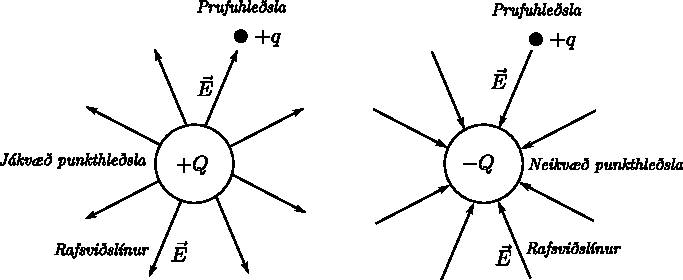
\includegraphics{prufuhledslur.pdf}
    \caption{Stefna rafsviðsins frá tveimur punkthleðslum með gagnstæð formerki.}
\end{figure}
\end{tcolorbox}

\begin{tcolorbox}
\begin{theorem}
\textbf{(Samlagningarlögmálið)} Ef rafsviðið sem að prufuhleðsla $q$ finnur fyrir frá mörgum punkthleðslum $Q_1, Q_2, \ldots, Q_n$ er gefið með $\vec{E}_1, \vec{E}_2, \ldots, \vec{E}_n$ þá er heildarrafsviðið sem prufuhleðslan finnur fyrir gefið með:
\begin{align*}
    \vec{E}_{\text{heild}} = \vec{E}_1 + \vec{E}_2 + \ldots + \vec{E}_n.
\end{align*}
\end{theorem}
\end{tcolorbox}

\textbf{Útleiðsla:} Þetta er bara einföld afleiðing af öðru lögmáli Newtons. Ef $\vec{F}_{\text{heild}}$ er heildarkrafturinn sem verkar á prufuhleðslu $q$ frá mörgum punkthleðslum $Q_1, Q_2, \ldots, Q_n$ sem hafa stefnuvigra $\vec{r}_1, \vec{r}_2, \ldots, \vec{r}_n$ þá er heildarrafsviðið gefið með:
\begin{align*}
    \vec{E}_{\text{heild}} = \frac{1}{q} \vec{F}_{\text{heild}} = \frac{1}{q}\left( \frac{kqQ_1}{r_1^2} \hat{\vec{r}}_1 + \frac{kqQ_2}{r_2^2} \hat{\vec{r}}_2 + \ldots + \frac{kqQ_n}{r_n^2} \hat{\vec{r}}_n \right) = \vec{E}_1 + \vec{E}_2 + \ldots + \vec{E}_n
\end{align*}
Þar sem $\vec{E}_n = \frac{kQ_n}{r_n^2} \hat{\vec{r}}_n$. \qed



\begin{tcolorbox}
\begin{theorem}
Lítum á eind með massa $m$ og hleðslu $q$ sem á verkar rafsvið $\vec{E}$. Þá finnur hún fyrir heildarkrafti:
\begin{align*}
    \vec{F}_{\text{heild}} = m\vec{a} = \vec{F}_{E} = q\vec{E}.
\end{align*}
\end{theorem}
\end{tcolorbox}

\textbf{Útleiðsla:} Við höfum þá að:
\begin{align*}
    \vec{F}_{\text{heild}} &= \vec{F}_1 + \vec{F}_2 + \ldots + \vec{F}_n \\
    &= \frac{kqQ_1}{r_1^2} \hat{\vec{r}}_1 + \frac{kqQ_2}{r_2^2} \hat{\vec{r}}_2 + \ldots + \frac{kqQ_n}{r_n^2} \hat{\vec{r}}_n \\
    &= q\vec{E}_1 + q\vec{E}_2 + \ldots + q \vec{E}_n \\
    &= q \vec{E}_{\text{heild}}.
\end{align*}
Við skrifum gjarnan $\vec{E}$ í staðinn fyrir $\vec{E}_{\text{heild}}$ og köllum kraftinn $\vec{F}_E = q\vec{E}$ \emph{rafkraftinn}. \qed



\section{Raftvískaut}

Einfaldasta sýnidæmið sem að við getum tekið er eftirfarandi: Lítum á tvær jafnstórar hleðslur með gagnstæð formerki $\pm q$ sem eru í fjarlægð $d$ frá hvor annarri. Þetta kemur fyrir mun oftar fyrir í náttúrunni en maður myndi halda (t.d. í vatnssameindinni $H_2 O$). 

\begin{figure}[H]
    \centering
    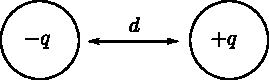
\includegraphics{tviskaut.pdf}
    \caption{Raftvískaut}
\end{figure}

Við höfum séð hvernig að hleðslurnar einar og sér mynda rafsvið í kringum sig. En hvernig lítur rafsviðið út þegar að við leggjum saman rafsviðin þeirra?

Til þess að teikna rafsviðslínur þá þurfum við að ímynda okkur að við höfum litla jákvæða prufuhleðslu. Síðan teiknum við rafsviðslínurnar út frá því hvernig heildarkrafturinn sem að prufuhleðslan myndi finna fyrir í þeim punkti lítur út. Það vill þannig til að rafsviðslínurnar sýna ferilinn sem að jákvæða prufuhleðslan myndi hreyfast eftir ef að henni væri sleppt þar.

\begin{figure}[H]
    \centering
    \begin{tikzpicture}
\path node[circle,inner sep=1ex] (L){} (5,0) node[circle,inner sep=1ex] (R){};
\foreach \X in {1,...,6}
 {\draw[very thick,attach arrow] (L) 
 to[out={-70+\X*20+8*rnd-4},in={180+70-\X*20+8*rnd-4},looseness=1.2] 
 (R);}
\foreach \X in {3,...,7}
 {\draw[very thick,attach arrow] (L) to[bend left=16-4*\X+2*rnd-4] ++ (70+\X*22:3);
 \draw[very thick,attach arrow] (R)+(180+70+\X*22:3) to[bend right=16-4*\X+2*rnd-4]
  (R);}
\path[inner color=white,outer color=black!30,shift={(L)}] 
 plot[smooth cycle,samples at={0,15,...,345}]
 (\x:{0.6});
\path[inner color=white,outer color=black!30,shift={(R)}] 
 plot[smooth cycle,samples at={0,15,...,345}]
 (\x:{0.6});
\path (L) node{$+q$} (R) node{$-q$} ;
\draw[thick,Stealth-] (0,2) -- (5,2);
\node at (0.5,1.5) {$\vec{\mu} = q\vec{d}$};
\end{tikzpicture}
    \caption{Rafsviðslínurnar í kringum tvískautið.}
\end{figure}

Það er reyndar stærð sem að fólk skilgreinir oft á þessum tímapunkti sem að kallast \emph{tvískautsvægið} og er táknað með $\vec{\mu}$ og skilgreint þannig að:
\begin{align*}
    \vec{\mu} = q \vec{d}
\end{align*}
Þar sem að $q$ er hleðsla raftvískautsins og $\vec{d}$ er vigurinn frá neikvæðu hleðslunni að þeirri jákvæðu. \\

Við skulum reyna að átta okkur betur á tvískautinu. Hugsum okkur að við komum neikvæðu hleðslu tvískautsins fyrir í $(0,0)$ í hnitakerfinu og jákvæðu hleðslunni í $(d,0)$. Okkur langar til þess að skoða hvert rafsviðið verður í $(x,0)$ langt í burtu $(x \gg d)$ á $x$-ás. Skoðum mynd af þessu:
 
\begin{figure}[H]
    \centering
\begin{tikzpicture}
        \draw (0,0) circle (0.5cm);
        \node at (0,0) {$-q$};
        \draw (3,0) circle (0.5cm);
        \node at (3,0) {$+q$};
        \draw[<->] (0.55,0) -- (2.45,0);
        \node at (1.5,0.3) {$d$};
        \node at (0,-0.9) {$(0,0)$};
        \node at (3,-0.9) {$(d,0)$};
        \draw[thick,|-Stealth] (0,1.5) -- (6,1.5);
        \node at (6.2,1.3) {$x$};
        \filldraw[draw=black] (6,0) circle (0.15cm);
        \node at (6,-0.5) {$(x,0)$};
        \node at (6,0.4) {$+e$};
        \draw[thick, -Stealth] (6,0) -- (7,0);
        \draw[thick, -Stealth] (6,0) -- (5.2,0);
        \node at (7.3,-0.3) {$\vec{E}_+$};
        \node at (5,-0.3) {$\vec{E}_-$};
\end{tikzpicture}
    \caption{Rafsviðið frá tvískautinu á prufuhleðslu $+e$ meðfram $x$-ás.}
\end{figure}
Við sjáum að rafsviðið í $(x,0)$ verður þá:
\begin{align*}
    \vec{E}_{\text{heild}} &= \vec{E}_+ + \vec{E}_- = \frac{kq}{(x-d)^2} - \frac{kq}{x^2}.
\end{align*}
Við getum umritað þetta aðeins til þess að koma þessu yfir á form þar sem að við getum notað uppáhaldsnálgun eðlisfræðingsins, þ.e.a.s.~tvíliðunálgunina $(1+b)^n \approx 1 + nb$ fyrir lítil $b \ll 1$.
\begin{align*}
    E_{\text{tvískaut}} = \frac{kq}{(x-d)^2} - \frac{kq}{x^2} = \frac{kq}{x^2}\left( \left(1 - \frac{d}{x} \right)^{-2} - 1 \right) \stackrel{d \ll x}{\approx} \frac{kq}{x^2}\left( 1 + \frac{2d}{x} - 1 \right) = \frac{2kqd}{x^3}.
\end{align*}
Þar sem að við höfum notað að stærðin $\frac{d}{x} \ll 1$ því $d \ll x$. Rafsviðið frá raftvískautinu fellur mjög hratt (eins og $1/x^3$). Langt í burtu frá tvískautinu þá er styrkur rafsviðsins næstum því núll! \\

En hvers vegna var stærðin $\vec{\mu} = q \vec{d}$ eiginlega kölluð tvískautsvægi? Hvaðan kemur tengingin við kraftvægið? Til þess að sjá það þá þurfum við að koma tvískautinu fyrir í utanaðkomandi rafsvið $\vec{E}$. Látum $\theta$ vera hornið sem að rafsviðið, $\vec{E}$ myndar við tvískautsvægið, $\vec{\mu}$:

\begin{figure}[H]
    \centering
\begin{tikzpicture}
\draw [-Stealth] (-2,0) -- (5,0);
\draw [-Stealth] (-2,-1) -- (5,-1);
\draw [-Stealth] (-2,-2) -- (5,-2);
\draw [-Stealth] (-2,1) -- (5,1);
\draw [-Stealth] (-2,2) -- (5,2);
\node at (5.2,1.3) {$\vec{E}$};
\draw[thick, rounded corners=15, rotate = 55, fill=white]
  (2,0) rectangle ++(-3,-1);
\node at (1.25,1) {$+q$};
\node at (0.15,-0.75) {$-q$};
\draw[thick,-Stealth] (1.6,1.3) -- (3,1.3);
\draw[thick,-Stealth] (-0.1,-1.15) -- (-1.5,-1.15);
\node at (3.2,1.5) {$\vec{F}_+$};
\node at (-1.5,-1.5) {$\vec{F}_-$};
\node at (2,0.35) {$\theta$};
\node at (0.9,0) {$\vec{\mu}$};
\draw[-{>[flex=0.75]}] (4,0.9) arc (65:-60:.4cm);
\node at (3.9,0.6) {$\vec{\tau}$};
\draw (1.75,0) arc (0:40:0.75cm);
\draw[thick,rotate = 55,-Stealth] (0,-0.5) -- (1,-0.5);
\end{tikzpicture}
    \caption{Tvískaut með tvískautsvægi $\vec{\mu} = q\vec{d}$ í ytra rafsviði $\vec{E}$.}
\end{figure}
Raftvískautið mun byrja að snúast um massamiðju sína. Við sjáum þá að kraftvægið sem að verkar á tvískautið er gefið með:
\begin{align*}
    \tau = F_+ \cdot \frac{d}{2}\sin\theta + F_- \cdot \frac{d}{2}\sin\theta = qEd\sin\theta = \mu E\sin\theta.
\end{align*}
Almennt gildir að:
\begin{align*}
    \vec{\tau} = \vec{\mu} \times \vec{E}.
\end{align*}

\section{Lagrange-punktar}

Þegar við skoðuðum þyngdarlögmálskraftinn þá sáum við að til voru punktar (sem kallast Lagrange-punktar) þar sem að heildarkrafturinn sem að verkar á hlut vegna tveggja annarra er núll (til dæmis einhversstaðar á milli jarðarinnar og tunglsins verður þyngdarlögmálskrafturinn sem að verkar á okkur núll). Fyrir rafkraftinn er þetta aðeins flóknara því að þá geta kraftarnir líka haft stefnur. Það eru í rauninni $2^3$ tilvik eftir því hvaða formerki hleðslurnar hafa. En til einföldunar skulum við skoða eitt ákveðið tilvik af þessum. Skoðum því sýnidæmi þar sem að við höfum hleðslu $+Q_1$ sem er stödd í $x = 0$ og aðra hleðslu $+Q_2$ sem er stödd í $x = r$. Hvar, $x$, ættum við að staðsetja litla, neikvæða hleðslu, $-q$ þannig að heildarkrafturinn sem að verkar á hana er núll?

\begin{figure}[H]
    \centering
\begin{tikzpicture}
        \draw (0,0) circle (0.5cm);
        \node at (0,0) {$+Q_1$};
        \draw (3,0) circle (0.5cm);
        \node at (3,0) {$-q$};
        \draw (5,0) circle (0.5cm);
        \node at (5,0) {$+Q_2$};
        \draw[<->] (0.55,0) -- (2.45,0);
        \node at (1.5,0.3) {$x_1$};
        \draw[<->] (3.55,0) -- (4.45,0);
        \node at (4,0.3) {$x_2$};
        \draw[<->] (0.55,-0.75) -- (4.45,-0.75);
        \node at (2.5,-1) {$r = x_1 + x_2$};
        \draw[thick,-Stealth] (3,1) -- (4,1);
        \draw[thick,-Stealth] (3,1) -- (2,1);
        \node at (2.5,1.25) {$F_1$};
        \node at (3.5,1.25) {$F_2$};
        \filldraw[draw=black] (3,1) circle (0.1cm);
\end{tikzpicture}
    \caption{Kraftajafnvægi fyrir hleðsluna $-q$ er einungis að finna á milli hleðslanna $+Q_1$ og $+Q_2$.}
\end{figure}

Einhverstaðar á milli hleðslanna munum við hafa:
\begin{align*}
    F_1 = F_2 \implies \frac{kQ_1 q}{x_1^2} = \frac{kQ_2 q}{x_2^2}
\end{align*}

En við höfum að $x_2 = r - x_1$, þannig að við fáum:
\begin{align*}
    \frac{Q_1}{x_1^2} = \frac{Q_2}{(r-x_1)^2} \implies \left( \frac{r-x_1}{x_1} \right)^2 = \frac{Q_2}{Q_1} \implies \frac{r}{x_1} - 1 = \pm \sqrt{\frac{Q_2}{Q_1}} \implies x_1 = \frac{r}{1 \pm \sqrt{\frac{Q_2}{Q_1}}}
\end{align*}

Þannig að ef við viljum að ögnin með hleðslu $-q$ sé í kraftajafnvægi á milli $+Q_1$ og $+Q_2$ þá þyrfti hún að vera í fjarlægð $x_1 = r/\left(1 \pm \sqrt{\frac{Q_2}{Q_1}}\right)$ frá hleðslunni $Q_1$. En þetta eru tvær lausnir! Hvernig stendur á því? Lausnin $x_1 = r/\left(1- \sqrt{\frac{Q_2}{Q_1}}\right)$ samsvarar því að $Q_1$ liggi á milli $Q_1$ og $Q_2$ og er því rétta lausnin. En $x_1 = r/\left(1 + \sqrt{\frac{Q_2}{Q_1}}\right)$ samsvarar því að ögninin liggi ekki á milli þeirra heldur hinum meginn við aðra hleðsluna! En það gengur ekki upp (það getur ekki verið neitt kraftajafnvægi fyrir utan hleðslurnar).



\section{Rafsviðið meðfram samhverfuás hringlaga gjarðar}

Við kynnum nú til sögunnar hleðsluþéttleikann. Við höfum áður talað um eðlismassa, $\rho = \frac{m}{V}$, þar sem að $m$ er massi hlutarins og $V$ er rúmmál hans. Þetta er massaþéttleiki. Við höfðum líka séð (þegar við vorum að glíma við staðbylgjur á streng) svokallaðan línulegan massaþéttleika, $\lambda = \frac{m}{\ell}$, þar sem að $m$ var massi vírsins og $\ell$ var lengd hans. Við kynnum því til sögunnar:


\begin{tcolorbox}
\begin{definition}
Lítum á hlut af lengd $L$, með yfirborðsflatarmál $A$ og rúmmál $V$. Látum $Q$ vera heildarhleðslu hlutarins. Við skilgreinum þá:
\begin{enumerate}[label = \textbf{(\roman*)}]
    \item Línulegan hleðsluþéttleiki hlutarins sem:
    \begin{align*}
        \lambda = \frac{Q}{L}.
    \end{align*}
    \item Yfirborðshleðsluþéttleiki hlutarins sem:
    \begin{align*}
        \sigma = \frac{Q}{A}.
    \end{align*}
    
    \item Hleðsluþéttleiki hlutarins sem:
    \begin{align*}
        \rho = \frac{Q}{V}.
    \end{align*}
\end{enumerate}
\end{definition}
\end{tcolorbox}

Við skulum síðan sýna hvernig þetta er notað. Hugmyndin er einfaldlega sú að sérhverja stóra hleðslu $Q$ getum við brotið niður í minni hleðslur $q$. Reyndar ef við viljum vera formleg þá er til heiltala $n \in \N$ þannig að $Q = n\cdot e$ þar sem $e$ er grunnhleðslan. En í sumum dæmum þar sem að við þekkjum ekki $n$ getur verið þægilegra að nota hleðsluþéttleikann (hann þjónar sama tilgangi). Við skulum sýna hvernig þetta er notað til þess að leiða út:

\begin{tcolorbox}
\begin{theorem}
Lítum á hringlaga gjörð með geisla $R$ og jafndreifða hleðslu $Q$ sem liggur í $yz$-planinu (jafna hringsins er þá $y^2 + z^2 = R^2$). Rafsviðið í punkti, $P = (x,0,0)$, í lóðréttri fjarlægð $x$ frá miðju gjarðarinnar er þá gefið með:
\begin{align*}
    E_x = kQ \cdot \frac{x}{(R^2 +x^2)^{3/2}}, \hspace{1cm} E_y = E_z = 0.
\end{align*}
\end{theorem}
\end{tcolorbox}
    
\begin{figure}[H]
    \centering
    \begin{tikzpicture}
    \draw[line width = 5pt, gray] (0,0) ellipse (1cm and 4cm);
    \draw[line width = 0.5pt, -Stealth] (0,0) -- (10,0);
    \draw[thick,-Stealth] (-4,-4) -- (-2.5,-4);
    \draw[thick,-Stealth] (-4,-4) -- (-4,-2.5);
    \draw[dashed] (0,0) -- (0,4);
    \draw[dashed] (0,4) -- (7,0);
    \draw[thick, fill=white] (-4,-4) circle (0.30cm);
    \draw[thick, fill=black] (-4,-4) circle (0.05cm);
    \draw[thick, fill=black] (7,0) circle (0.1cm);
    \draw[thick, fill=black] (0,4) circle (0.1cm);
    \draw (6,0) arc (180:150:1cm);
    \node at (-2.3,-4.25) {$x$};
    \node at (-3.7,-2.3) {$y$};
    \node at (-4.5,-4) {$z$};
    \node at (-0.4,2) {$R$};
    \node[rotate=-30] at (3,3) {$r = \sqrt{R^2 + x^2}$};
    \node at (3.5,-0.4) {$x$};
    \node at (-1.25,-2.75) {$Q$};
    \node at (0.8,4.3) {$dq = \lambda d\ell$};
    \node at (7.75,0.45) {$P = (x,0,0)$};
    \node at (5.75,0.30) {$\theta$};
    \node at (8.75,-2) {$d\vec{E}$};
    \node at (2,-3) {$\lambda = \frac{Q}{2\pi R}$};
    \draw[thick, -Stealth] (7,0) -- (9,-1.5);
    \end{tikzpicture}
\end{figure}

\textbf{Útleiðsla:} Skoðum lítinn bút af gjörðinni af lengd $d\ell$. Línulegur hleðsluþéttleiki gjarðarinnar er $\lambda = \frac{Q}{2\pi r}$. Þá er hleðslan í þessum litla bút $d\ell$ gefin með $dq = \lambda d\ell$. Við getum litið á þessa litlu hleðslu sem punkthleðslu (gætum, ef við vildum, valið $d\ell$ þannig að $dq$ verður jöfnu grunnhleðslunni $e$). Hvert er þá framlag litlu hleðslunnar $dq$ til rafsviðsins í punktinum $P = (x,0,0)$? Litla hleðslan $dq$ gefur framlag $d\vec{E}$ til rafsviðsins. Við vitum að heildarrafsviðið verður einungis í $x$-stefnuna (styttist út í $y$ og $z$ stefnurnar vegna samhverfu) svo að við þurfum einungis að reikna þann þátt af $d\vec{E}$ sem er samsíða $x$-ásnum. Fáum þá:
\begin{align*}
    dE_x = \abs{d\vec{E}} \cos\theta = \abs{d\vec{E}} \cdot \frac{x}{\sqrt{R^2 + x^2}}
\end{align*}
En við höfum að:
\begin{align*}
    \abs{d\vec{E}} = \frac{kdq}{R^2 + x^2}, \hspace{1cm} \text{þ.a.~} \hspace{1cm} dE_x = \abs{d\vec{E}} \cdot \frac{x}{\sqrt{R^2 + x^2}} = \frac{kxdq}{\left(R^2 + x^2 \right)^{3/2}}
\end{align*}
Síðan þurfum við að leggja saman öll þessi framlög frá öllum litlu hleðslunum $dq = \lambda d\ell$ í gjörðinni. En þá höfum við að:
\begin{align*}
    E_x = \int dE_x = \int \frac{kxdq}{(R^2 + x^2)^{3/2}} = \int \frac{kx\lambda d\ell}{(R^2 + x^2)^{3/2}} = \frac{kx\lambda}{(R^2 + x^2)^{3/2}} \explain{\int d\ell }{2\pi R} = \frac{2\pi R k x \lambda}{(R^2 + x^2)^{3/2}}.
\end{align*}
  
Ef við rifjum síðan upp að $\lambda = \frac{Q}{2\pi R}$ þá sjáum við að lokum að:
\begin{align*}
    E_x = kQ \cdot \frac{x}{(R^2 + x^2)^{3/2}}
\end{align*}

Til að sannreyna svarið okkar þá getum við athugað að ef $x \gg R$ þá höfum við að rafsviðið verður: $E_x \approx \frac{kQ}{x^2}$ eins og við er að búast því þá lítur gjörðin út eins og punkthleðsla með hleðslu $Q$.
  

\section{Rafsviðið frá óendanlega stórri plötu (*)}
Lítum á plötu með hleðsluþéttleika $\sigma$. Ef platan er óendanlega stór þá er auðvelt að sannfæra sig um að rafsviðið sé einungis í stefnuna frá plötunni (þ.e.~ef platan er í $xy$-planinu þá er rafsviðið einungis með $z$-þátt) Höfum þá að á $z$-ásnum þá er framlagið frá litlum bút með flatarmál $dxdy$:
\begin{align*}
    dE_z = \frac{kdq}{(x^2+y^2 + z^2)^{3/2}}\cdot z = \frac{kz\sigma dx dy}{(x^2+y^2+z^2)^{3/2}}
\end{align*}
Þannig að:
\begin{align*}
    E_z &= \int dE_z = \int_{-\infty}^{+\infty} \int_{-\infty}^{+\infty} \frac{kz\sigma}{(x^2+y^2+z^2)}dxdy \\ &= 4\int_{0}^{+\infty} \int_{0}^{+\infty} \frac{kz\sigma}{(x^2+y^2+z^2)}dxdy \\
    &= 4 \int_{0}^{+\infty} \left[ \frac{kz\sigma x dy}{(y^2+z^2)\sqrt{x^2+y^2+z^2}} \right]_{0}^{+\infty} dy \\
    &= 4 \int_{0}^{+\infty} \frac{kz\sigma}{(y^2+z^2)}dy \\
    &= \frac{4kz\sigma}{z} \left[ \arctan(\frac{y}{z}) \right]_{0}^{+\infty} \\
    &= 4k\sigma \left( \arctan(\infty) - \arctan(0) \right) \\
    &= 2k\sigma \left( \frac{\pi}{2} - 0 \right) \\
    &= 2\pi k \sigma
\end{align*}
En síðan rifjum við upp að $k = \frac{1}{4\pi \varepsilon_0}$ þ.a.~
\begin{align*}
    E_z = \frac{\sigma}{2\varepsilon_0} = \frac{Q}{2\varepsilon_0 A}
\end{align*}
Sem er vissulega óháð $z$ ef platan er óendnanlega stór!

\newpage

\section{Dæmi}

\subsection*{Dæmatími 1: Coulombskrafturinn}

\begin{tcolorbox}
Coulombskrafturinn (eða rafkrafturinn) sem verkar á milli tveggja hleðsla $q_1$ og $q_2$ sem eru í fjarlægð $r$ frá hver er gefinn með:
\begin{align*}
    \vec{F}_k = \frac{kq_1 q_2}{r^2} \hat{r}.
\end{align*}
þar sem $k = \SI{8.98e9}{N.m^2/C^2}$ er fasti sem nefnist fasti Coulombs og $\hat{r}$ táknar einingarvigur í stefnuna frá annarri hleðslunni til hinnar. Krafturinn er fráhrindikraftur ef hleðslurnar hafa sama formerki en aðdráttarkraftur ef hleðslurnar hafa sama formerki.
\end{tcolorbox}

\begin{enumerate}[label = \textbf{(\alph*)}]
    \item[\textbf{(22.13)}] Lítum á tvo jafnstóra massa $m = m_1 = m_2 = \SI{2}{kg}$ með jafnstóra jákvæða hleðslu $q = Q_1 = Q_2 = +\SI{5}{mC}$ sem eru í fjarlægð $d = \SI{1}{m}$ frá hvor öðrum á núningslausu borði.
    \begin{enumerate}[label = \textbf{(\alph*)}]
        \item Hver er stærð Coulombskraftsins/rafkraftsins sem verkar á annan hvorn massann?
        \item Nú er mössunum sleppt úr kyrrstöðu. Hver verður hröðun massanna einmitt á því augnabliki?
    \end{enumerate}
    
    \item[\textbf{(22.16)}] Tvær róteindir með massa $m_p = \SI{1.67e-27}{kg}$ og með hleðslu $+e = \SI{+1.602e-19}{C}$ eru staddar í fjarlægð $r = \SI{1}{fm}$ frá hver annarri.
    \begin{enumerate}[label = \textbf{(\alph*)}]
        \item Hver er stærð Coulombskraftsins, $F_k$, sem að önnur róteindin verkar með á hina?
        \item Hver er stærð þyngdarlögmálskraftsins, $F_G$, sem að önnur róteindin verkar með á hina?
        \item Hverrt er hlutfallið $\frac{F_k}{F_G}$?
    \end{enumerate}
    
    \item[\textbf{(22.17)}] Lítum á eftirfarandi mynd:
    \begin{figure}[H]
        \centering
        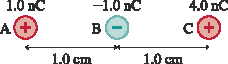
\includegraphics[scale = 1.25]{figures/rk-charges.pdf}
    \end{figure}
    Hver er heildarkrafturinn sem að verkar á hleðsluna A?
    
    \item[\textbf{(22.19)}] Lítum á eftirfarandi mynd:
    \begin{figure}[H]
        \centering
        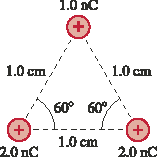
\includegraphics[scale = 1.25]{figures/rk2219.pdf}
    \end{figure}
    Hver er heildarkrafturinn sem að verkar á hleðsluna A?
\end{enumerate}


\begin{tcolorbox}
\begin{enumerate*}[label = \vspace{0.15cm} ]
  \item \textbf{(22.13)} $F_k = \SI{200}{kN}$, $a = \SI{1e5}{m/s^2}$.
  \item \textbf{(22.16)} $F_k = \SI{230}{N}$, $F_G = \SI{1.9e-34}{N}$, $\frac{F_k}{F_G} = \SI{1.2e36}{}$.
  \item \textbf{(22.17)} $\Vec{F}_{\text{heild}} = \vec{0}$.
  \item \textbf{(22.19)} $\displaystyle \vec{F}_{\text{heild}} = \smqty(0 \\ \SI{3.1e-4}{}) \, \si{N}$.
\end{enumerate*}
\end{tcolorbox}

\subsection*{Dæmatími 2: Rafsviðið}

\begin{tcolorbox}
Rafsviðið sem að punkthleðsla $Q$ myndar í kringum sig í fjarlægð $r$ frá henni er gefið með:
\begin{align*}
    \vec{E} = \frac{kQ}{r^2}\hat{r}
\end{align*}
þar sem $\hat{r}$ er einingarvigur í stefnuna frá punkthleðslunni að þeim stað þar sem að rafsviðið er metið. Við ímyndum okkur að við höfum komið fyrir jákvæðri punkthleðslu með litla hleðslu, $+q$, í þeim punkti þar sem að við viljum meta rafsviðið. Síðan skoðum við rafkraftinn sem að prufuhleðslan $+q$ myndi finna fyrir í þeim punkti og deilum loks með prufuhleðslunni, $+q$.
\end{tcolorbox}

\begin{enumerate}[label = \textbf{(\alph*)}]

\item[\textbf{(22.26)}] Hvert er rafsviðið í $r = \SI{1.0}{mm}$ fjarlægð frá \textbf{(a)} róteind \textbf{(b)} rafeind?

\item[\textbf{(22.26)}] Hleðsla $Q = +\SI{12}{nC}$ er staðsett í upphafspunkti hnitakerfis, $(\SI{0.0}{cm}, \SI{0.0}{cm})$. Hvert er rafsviðið í punktunum $A = (\SI{5.0}{cm}, \SI{0.0}{cm})$, $B = (\SI{-5.0}{cm}, \SI{5.0}{cm})$ og $C = (\SI{-5.0}{cm}, \SI{-5.0}{cm})$?

\item[\textbf{(22.63)}] Lítum á eftirfarandi mynd:

\begin{figure}[H]
    \centering
    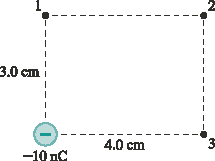
\includegraphics{figures/rk2263.pdf}
\end{figure}
Hvert er rafsviðið í $1$, $2$ og $3$?

\item[\textbf{(22.67)}] Lítum á ögn í rafsviði $\vec{E} = \smqty(100 \\ 0) \, \si{kN/C}$. Ögnin hefur massa $m = \SI{5.0}{g} = \SI{5.0e-3}{kg}$ og hangir kyrr undir horni $\theta = \ang{20}$ miðað við lárétt:
\begin{figure}[H]
    \centering
    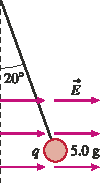
\includegraphics{figures/rk2267.pdf}
\end{figure}
Hver er hleðsla agnarinnar, $q$?

\end{enumerate}

\begin{tcolorbox}
\begin{enumerate*}[label = \vspace{0.15cm} ]
  \item \textbf{(22.26)} $E = \SI{1.4e-9}{N/C}$.
  \item \textbf{(22.32)} $E_A = \smqty(43 \\ 0) \, \si{kN/C}$, $E_B = \smqty(-15 \\ 15) \, \si{kN/C}$, $E_C = \smqty(-15 \\ -15) \, \si{kN/C}$.
    \item \textbf{(22.63)} $\vec{E}_1 = \smqty(0 \\ -100) \, \si{kN/C}$, $\vec{E}_2 = \smqty(-56 \\ 0) \, \si{kN/C}$, $\vec{E}_3 = \smqty(-29 \\ 22) \, \si{kN/C}$.
  \item \textbf{(22.67)} $q = \SI{180}{nC}$.
\end{enumerate*}
\end{tcolorbox}

\newpage

\subsection*{Dæmatími 3: Rafkrafturinn}

\begin{tcolorbox}
Hlaðin eind með hleðslu $q$ sem er stödd í utanaðkomandi rafsviði $\vec{E}$ (okkur er alveg sama hvernig þetta rafsvið varð til!) finnur fyrir rafkrafti:
\begin{align*}
    \vec{F}_E = q \vec{E}
\end{align*}
Takið eftir að jákvæðar eindir vilja ferðast með rafsviðslínunum en neikvæðar eindir vilja ferðast á móti rafsviðslínunum.
\end{tcolorbox}

\begin{enumerate}[label = \textbf{(\alph*)}]

\item[\textbf{(22.5)}] Hver er heildarhleðsla allra rafeindanna í \SI{1.0}{L} af vatni?

\item[\textbf{(22.54)}] Í einföldu líkani af vetnisatóminu þá er rafeindin á hringhreyfingu með geisla $r = \SI{0.053}{nm}$ umhverfis kyrrstæða róteind. Hversu margar umferðir fer rafeindin í kringum róteindina á sekúndu?

\item[\textbf{(22.73)}] Lítum á eftirfarandi mynd:

\begin{figure}[H]
    \centering
    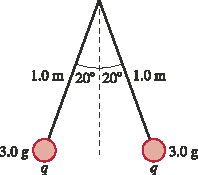
\includegraphics{figures/rk2273.pdf}
\end{figure}

Ákvarðið hleðsluna, $q$.

\item[\textbf{(22.75)}] Lítum á eftirfarandi mynd:

\begin{figure}[H]
    \centering
    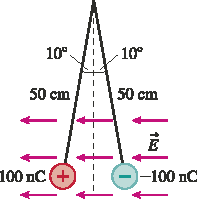
\includegraphics{figures/rk2275.pdf}
\end{figure}

Ákvarðið massann, $m$.

\end{enumerate}

\begin{tcolorbox}
\begin{enumerate*}[label = \vspace{0.15cm} ]
  \item \textbf{(22.5)} $Q \approx \SI{-5e7}{C}$.
  \item \textbf{(22.54)} $N = \SI{6.6e15}{snú/sek}$.
  \item \textbf{(22.73)} $q = \SI{750}{nC}$.
  \item \textbf{(22.75)} $m = \SI{5.8}{g}$.
\end{enumerate*}
\end{tcolorbox}

\newpage

%%%%%%%%%%%%%%%%%%%%%%%%%%%%%%%%
%      END OF CHAPTER TEXT 
%%%%%%%%%%%%%%%%%%%%%%%%%%%%%%%%
\ifdefined \wholebook \else
 \printindex
\end{document}
\fi
